\documentclass{article}

\usepackage{fancyhdr}
\usepackage{extramarks}
\usepackage{amsmath}
\usepackage{amsthm}
\usepackage{amsfonts}
\usepackage{tikz}
\usepackage[plain]{algorithm}
\usepackage{algpseudocode}
\usepackage{fancybox}

\usetikzlibrary{automata,positioning}

%
% Basic Document Settings
%

\topmargin=-0.45in
\evensidemargin=0in
\oddsidemargin=0in
\textwidth=6.5in
\textheight=9.0in
\headsep=0.25in

\linespread{1.1}

\pagestyle{fancy}
\lhead{\hmwkAuthorName}
\chead{\hmwkClass\ (\hmwkClassInstructor\ \hmwkClassTime): \hmwkTitle}
\rhead{\firstxmark}
\lfoot{\lastxmark}
\cfoot{\thepage}

\renewcommand\headrulewidth{0.4pt}
\renewcommand\footrulewidth{0.4pt}

\setlength\parindent{0pt}

%
% Create Problem Sections
%

\newcommand{\enterProblemHeader}[1]{
    \nobreak\extramarks{}{Problem \arabic{#1} continued on next page\ldots}\nobreak{}
    \nobreak\extramarks{Problem \arabic{#1} (continued)}{Problem \arabic{#1} continued on next page\ldots}\nobreak{}
}

\newcommand{\exitProblemHeader}[1]{
    \nobreak\extramarks{Problem \arabic{#1} (continued)}{Problem \arabic{#1} continued on next page\ldots}\nobreak{}
    \stepcounter{#1}
    \nobreak\extramarks{Problem \arabic{#1}}{}\nobreak{}
}

\setcounter{secnumdepth}{0}
\newcounter{partCounter}
\newcounter{homeworkProblemCounter}
\setcounter{homeworkProblemCounter}{1}
\nobreak\extramarks{Problem \arabic{homeworkProblemCounter}}{}\nobreak{}

%
% Homework Problem Environment
%
% This environment takes an optional argument. When given, it will adjust the
% problem counter. This is useful for when the problems given for your
% assignment aren't sequential. See the last 3 problems of this template for an
% example.
%
\newenvironment{homeworkProblem}[1][-1]{
    \ifnum#1>0
        \setcounter{homeworkProblemCounter}{#1}
    \fi
    \section{Problem \arabic{homeworkProblemCounter}}
    \setcounter{partCounter}{1}
    \enterProblemHeader{homeworkProblemCounter}
}{
    \exitProblemHeader{homeworkProblemCounter}
}

%
% Homework Details
%   - Title
%   - Due date
%   - Class
%   - Section/Time
%   - Instructor
%   - Author
%

\newcommand{\hmwkTitle}{Homework\ \#1}
\newcommand{\hmwkDueDate}{October 8, 2019}
\newcommand{\hmwkClass}{CS251}
\newcommand{\hmwkClassTime}{Section A}
\newcommand{\hmwkClassInstructor}{Steven Libby}
\newcommand{\hmwkAuthorName}{\textbf{Austen Nelson}}

%
% Title Page
%

\title{
    \vspace{2in}
    \textmd{\textbf{\hmwkClass:\ \hmwkTitle}}\\
    \normalsize\vspace{0.1in}\small{Due\ on\ \hmwkDueDate\ at 2:00pm}\\
    \vspace{0.1in}\large{\textit{\hmwkClassInstructor\ \hmwkClassTime}}
    \vspace{3in}
}

\author{\hmwkAuthorName}
\date{}

\renewcommand{\part}[1]{\textbf{\large Part \Alph{partCounter}}\stepcounter{partCounter}\\}

%
% Various Helper Commands
%

% Useful for algorithms
\newcommand{\alg}[1]{\textsc{\bfseries \footnotesize #1}}

% For derivatives
\newcommand{\deriv}[1]{\frac{\mathrm{d}}{\mathrm{d}x} (#1)}

% For partial derivatives
\newcommand{\pderiv}[2]{\frac{\partial}{\partial #1} (#2)}

% Integral dx
\newcommand{\dx}{\mathrm{d}x}

% Alias for the Solution section header
\newcommand{\solution}{\textbf{\large Solution}}

% Probability commands: Expectation, Variance, Covariance, Bias
\newcommand{\E}{\mathrm{E}}
\newcommand{\Var}{\mathrm{Var}}
\newcommand{\Cov}{\mathrm{Cov}}
\newcommand{\Bias}{\mathrm{Bias}}

% these are several symbols that I redefined to make formulas easier to read
\def\land{\wedge}           % /\
\def\lor{\vee}              % \/
\def\lnot{\neg}             % -
\def\liff{\leftrightarrow}  % <->
\def\xor{\oplus}            % (+)
\def\T{\top}                % T
\def\F{\bot}                % _|_

\begin{document}

\maketitle

\pagebreak

\begin{homeworkProblem}
   Define variables, and write the following sentences as logical statements.\\

   \textbf{Part One}\\
   Sentence: If it's not cloudy, then it's not raining.\\
   Variables:
\begin{itemize}
    \item A --- It is cloudy.
    \item B --- It is raining.
\end{itemize}
   Statement: $\lnot A \to \lnot B$
   \vspace{1cm}

   \textbf{Part Two}\\
   Sentence: If we won the big game, then either we scored more points, or the other team didn't show up.\\
   Variables:
\begin{itemize}
    \item A --- We won the big game.
    \item B --- We scored more points.
    \item C --- The other team showed up.
\end{itemize}
   Statement: $A \to (B \lor \lnot C)$
   \vspace{1cm}

   \textbf{Part Three}\\
   Sentence: This is a sentence.\\
   Variables:
\begin{itemize}
    \item A --- This is a sentence.
\end{itemize}
   Statement: $A$
   \vspace{1cm}

   \textbf{Part Four}\\
   Sentence: If you don't study for tests, then you won't pass the class.\\
   Variables:
\begin{itemize}
    \item A --- You study for tests.
    \item B --- You pass the class.
\end{itemize}
   Statement: $\lnot A \to \lnot B$
   \vspace{1cm}

   \textbf{Part Five}\\
   Sentence: A graph is planer if it contains neither a minor of $K_{3,3}$ nor $K_5$.\\
   Variables:
\begin{itemize}
   \item A --- A graph contains a minor of $K_{3,3}$.
   \item B --- A graph contains a minor of $K_5$.
   \item C --- A graph is planer.
\end{itemize}
   Statement: $(\lnot A \land \lnot B) \to C$
\end{homeworkProblem}

\begin{homeworkProblem}
Draw truth tables for the following formulas.\\

$a \xor b$
$$
\begin{array}{|c|c||c|}
  \hline
  a  & b  & a \xor b \\
  \hline
  1  & 1  &    0     \\
  \hline
  1  & 0  &    1     \\
  \hline
  0  & 1  &    1     \\
  \hline
  0  & 0  &    0     \\
  \hline
\end{array} 
$$
$\lnot (\lnot a)$
$$
\begin{array}{|c||c|}
  \hline
  a  & \lnot (\lnot a) \\
  \hline
  1  &        1        \\
  \hline
  0  &        0        \\
  \hline
\end{array} 
$$
$\lnot b \to \lnot a$
$$
\begin{array}{|c|c||c|}
  \hline
  a  & b  & \lnot a \to \lnot b   \\
  \hline
  1  & 1  &          1            \\
  \hline
  1  & 0  &          1            \\
  \hline
  0  & 1  &          0            \\
  \hline
  0  & 0  &          1            \\
  \hline
\end{array} 
$$
$\lnot a \land \lnot b$
$$
\begin{array}{|c|c||c|}
  \hline
  a  & b  & \lnot a \land \lnot b \\
  \hline
  1  & 1  &          0            \\
  \hline
  1  & 0  &          0            \\
  \hline
  0  & 1  &          0            \\
  \hline
  0  & 0  &          1            \\
  \hline
\end{array} 
$$
$a \liff (b \liff c)$
$$
\begin{array}{|c|c|c||c|}
  \hline
  a  & b  & c  & a \liff (b \liff c) \\
  \hline
  1  & 1  & 1  &          1          \\
  \hline
  1  & 1  & 0  &          0          \\
  \hline
  1  & 0  & 1  &          0          \\
  \hline
  1  & 0  & 0  &          1          \\
  \hline
  0  & 1  & 1  &          0          \\
  \hline
  0  & 1  & 0  &          1          \\
  \hline
  0  & 0  & 1  &          1          \\
  \hline
  0  & 0  & 0  &          0          \\
  \hline
\end{array} 
$$
$(a \lor c) \land (b \lor c)$
$$
\begin{array}{|c|c|c||c|}
  \hline
  a  & b  & c  & (a \lor c) \land (b \lor c) \\
  \hline
  1  & 1  & 1  &              1              \\
  \hline
  1  & 1  & 0  &              1              \\
  \hline
  1  & 0  & 1  &              1              \\
  \hline
  1  & 0  & 0  &              0              \\
  \hline
  0  & 1  & 1  &              1              \\
  \hline
  0  & 1  & 0  &              0              \\
  \hline
  0  & 0  & 1  &              1              \\
  \hline
  0  & 0  & 0  &              0              \\
  \hline
\end{array} 
$$
\end{homeworkProblem}

\begin{homeworkProblem}
   Reduce the following to the shortest form.\\
   Determine if it's satisfiable, a tautology, or neither.\\

   \textbf{Part One}\\
   $(a \land \lnot b) \lor \lnot (\lnot a \lor b)$: satisfiable\\
   \begin{align*}
      &(a \land \lnot b) \lor \lnot (\lnot a \lor b)      && \\
      &(a \land \lnot b) \lor (a \land \lnot b)           && DM_{\lor}\\
      &a \land \lnot b                                    && Item_{\land}\\
      &\lnot \lnot (a \land \lnot b)                      && \lnot \lnot\\
      &\lnot (\lnot a \lor b)                             && DM_{\land}\\
      &\lnot (a \to b)                                    && Imp
   \end{align*}

   \textbf{Part Two}\\
   $a \land b \equiv \lnot (\lnot a \land \lnot b)$: satisfiable\\
   \begin{align*}
      &a \land b \equiv \lnot (\lnot a \land \lnot b)             &&\\
      &((a \land b) \to \lnot (\lnot a \land \lnot b))
      \land (\lnot (\lnot a \land \lnot b) \to (a \land b))       && Def \equiv\\
      &((a \land b) \to (a \lor b))
      \land (\lnot (\lnot a \land \lnot b) \to (a \land b))       && DM_{\land}\\
      &(\lnot (a \land b) \lor (a \lor b))
      \land (\lnot (\lnot a \land \lnot b) \to (a \land b))       && Imp\\
      &((\lnot a \lor \lnot b) \lor (a \lor b))
      \land (\lnot (\lnot a \land \lnot b) \to (a \land b))       && DM_{\land}\\
      &(\lnot a \lor a \lor \lnot b \lor b)
      \land (\lnot (\lnot a \land \lnot b) \to (a \land b))       && Com_{\lor}\\
      &( T \lor T)
      \land (\lnot (\lnot a \land \lnot b) \to (a \land b))       && LEM * 2\\
      &\lnot (\lnot a \land \lnot b) \to (a \land b)              && Id_{\land}\\
      &\lnot \lnot (\lnot a \land \lnot b) \lor (a \land b)       && Imp\\
      &(\lnot a \land \lnot b) \lor (a \land b)                   && \lnot \lnot\\
      &((\lnot a \land \lnot b) \lor a)
      \land ((\lnot a \land \lnot b) \lor b)                      && Dis_{\lor}\\
      &(a \lor (\lnot a \land \lnot b))
      \land (b \lor (\lnot a \land \lnot b))                      && Com_{\lor} * 2\\
      &((a \lor \lnot a) \land (a \lor \lnot b))
      \land (b \lor (\lnot a \land \lnot b))                      && Dis_{\lor}\\
      &(T \land (a \lor \lnot b))
      \land (b \lor (\lnot a \land \lnot b))                      && LEM\\
      &(a \lor \lnot b)
      \land (b \lor (\lnot a \land \lnot b))                      && Id_{\land}\\
      &(\lnot b \lor a)
      \land (b \lor (\lnot a \land \lnot b))                      && Com_{\lor}\\
      &(b \to a)
      \land (b \lor (\lnot a \land \lnot b))                      && Imp\\
      &(b \to a)
      \land ((b \lor \lnot a) \land (b \lor \lnot b))             && Dis_{\lor}\\
      &(b \to a)
      \land  (b \lor \lnot a) \land T                             && LEM\\
      &(b \to a)
      \land  (b \lor \lnot a)                                     && Id_{\land}\\
      &(b \to a)
      \land  (\lnot a \lor b)                                     && Com_{\lor}\\
      &(b \to a)
      \land (a \to b)                                             && Imp\\
      &a \equiv b                                                 && Def \equiv
   \end{align*}
   \pagebreak\\
   \textbf{Part Three}\\
   $a \land b \equiv \lnot (\lnot a \lor \lnot b)$: tautology\\ 
   \begin{align*}
      &a \land b \equiv \lnot (\lnot a \lor \lnot b)              &&\\
      &((a \land b) \to \lnot (\lnot a \lor \lnot b))
      \land (\lnot (\lnot a \lor \lnot b) \to (a \land b))        && Def \equiv\\
      &(\lnot (a \land b) \lor \lnot (\lnot a \lor \lnot b))
      \land (\lnot (\lnot a \lor \lnot b) \to (a \land b))        && Imp\\
      &((\lnot a \lor \lnot b) \lor \lnot (\lnot a \lor \lnot b))
      \land (\lnot (\lnot a \lor \lnot b) \to (a \land b))        && DM_{\land}\\
      &((\lnot a \lor \lnot b) \lor (a \land b))
      \land (\lnot (\lnot a \lor \lnot b) \to (a \land b))        && DM_{\lor}\\
      &(((\lnot a \lor \lnot b) \lor a) \land 
      ((\lnot a \lor \lnot b) \lor b))
      \land (\lnot (\lnot a \lor \lnot b) \to (a \land b))        && Dis_{\lor}\\
      &((\lnot a \lor a \lor \lnot b) \land 
      (\lnot a \lor \lnot b \lor b))
      \land (\lnot (\lnot a \lor \lnot b) \to (a \land b))        && Com_{\lor}\\
      &((T \lor \lnot b) \land (\lnot a \lor T))
      \land (\lnot (\lnot a \lor \lnot b) \to (a \land b))        && LEM * 2\\
      &T \land T
      \land (\lnot (\lnot a \lor \lnot b) \to (a \land b))        && Anul_{\lor} * 2\\
      &\lnot (\lnot a \lor \lnot b) \to (a \land b)               && Id_{\land}\\
      &(a \land b) \to (a \land b)                                && DM_{\lor}\\
      &T                                                          && Def \to
   \end{align*}

   \textbf{Part Four}\\
   $a \land (b \lor c) \to a \land (b \land c)$: satisfiable\\
   On the left hand side of the implication we have $a \land E$, where E is some expression.
   Because false always implies true, and when a is false $a \land E = F$ $(Anul_{\land})$, the
   expression $a \land (b \lor c) \to a \land (b \land c)$ will always be true when a is false.
   Using this knowledge we can reduce the expression to $\lnot a \lor (T \land (b \lor c) \to
   T \land (b \land c))$.
   \begin{align*}
      &\lnot a \lor (T \land (b \lor c) \to T \land (b \land c))  &&\\
      &\lnot a \lor (b \lor c \to b \land c)                      &&Id_{\land} * 2\\
      &\lnot a \lor (\lnot (b \lor c) \lor (b \land c))           &&Imp\\
      &\lnot a \lor ((\lnot b \land \lnot c) \lor (b \land c))    &&DM_{\lor}\\
      &\lnot a \lor
      (((\lnot b \land \lnot c) \lor b)
      \land ((\lnot b \land \lnot c) \lor c))                     &&Dis_{\lor}\\
      &\lnot a \lor
      ((b \lor (\lnot b \land \lnot c))
      \land (c \lor (\lnot b \land \lnot c)))                     &&Com_{\lor} * 2\\
      &\lnot a \lor
      (((b \lor \lnot b) \land (b \lor \lnot c))
      \land ((c \lor \lnot b) \land (c \lor \lnot c)))            &&Dis_{\lor} * 2\\
      &\lnot a \lor
      ((T \land (b \lor \lnot c))
      \land ((c \lor \lnot b) \land T))                           &&LEM * 2\\
      &\lnot a \lor
      ((b \lor \lnot c)
      \land (c \lor \lnot b))                                     &&Id_{\land} * 2\\
      &\lnot a \lor
      ((\lnot c \lor b)
      \land (\lnot b \lor c))                                     &&Com_{\lor} * 2\\
      &\lnot a \lor
      ((c \to b)
      \land (b \to c))                                            &&Imp * 2\\
      &\lnot a \lor
      (b \equiv c)                                                &&Def \equiv
   \end{align*}
\end{homeworkProblem}
\begin{homeworkProblem}
   Draw the following abstract syntax trees:\\
    \begin{figure}[h]
    \centering
    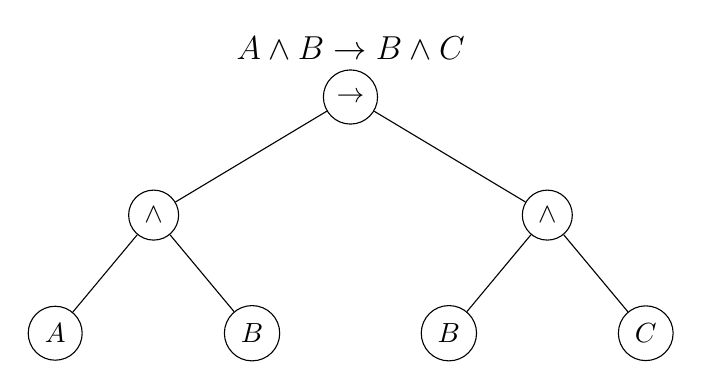
\begin{tikzpicture} [level/.style={sibling distance=50mm/#1}],
       \node [circle,draw] { $\to$ }
         child { node [circle,draw] { $\land$ }
            child { node [circle,draw] { $A$ } }
            child { node [circle,draw] { $B$ } } }
         child { node [circle,draw] { $\land$ }
            child { node [circle,draw] { $B$ } }
            child { node [circle,draw] { $C$ } } };
       \node[above,font=\large\bfseries] at (current bounding box.north) {$A \land B \to B \land C$};
    \end{tikzpicture}
    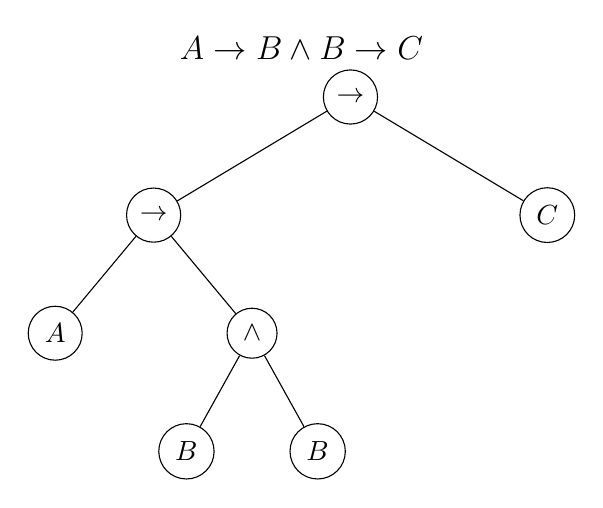
\begin{tikzpicture} [level/.style={sibling distance=50mm/#1}],
       \node [circle,draw] { $\to$ }
         child { node [circle,draw] { $\to$ }
            child { node [circle,draw] { $A$ } }
            child { node [circle,draw] { $\land$ } 
               child { node [circle,draw] { $B$ } }
               child { node [circle,draw] { $B$ } } } }
         child { node [circle,draw] { $C$ } };
       \node[above,font=\large\bfseries] at (current bounding box.north) {$A \to B \land B \to C$};
    \end{tikzpicture}
    \end{figure}
    \begin{figure}
    \centering
    \begin{tikzpicture} [level/.style={sibling distance=50mm/#1}],
       \node [circle,draw] { $\to$ }
         child { node [circle,draw] { $\lor$ }
            child { node [circle,draw] { $\land$ } 
               child { node [circle,draw] { $\lnot$ }
                  child { node [circle,draw] { $A$ } } }
               child { node [circle,draw] { $B$ } } }
            child { node [circle,draw] { $C$ } } }
         child { node [circle,draw] { $D$ } };
       \node[above,font=\large\bfseries] at (current bounding box.north) { $\lnot A \land B \lor C \to D$ };
    \end{tikzpicture}
    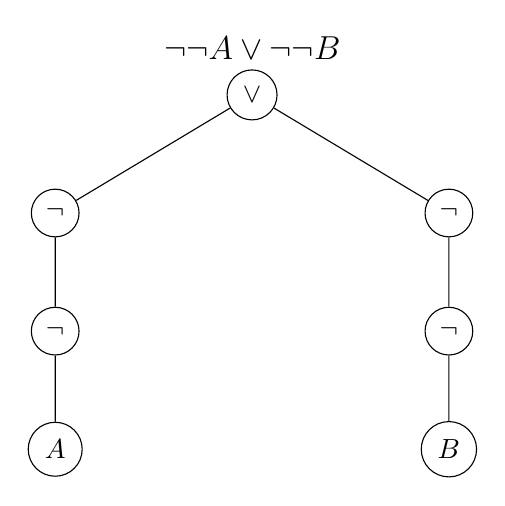
\begin{tikzpicture} [level/.style={sibling distance=50mm/#1}],
       \node [circle,draw] { $\lor$ }
         child { node [circle,draw] { $\lnot$ }
            child { node [circle,draw] { $\lnot$ } 
               child { node [circle,draw] { $A$ } } } }
         child { node [circle,draw] { $\lnot$ }
            child { node [circle,draw] { $\lnot$ } 
               child { node [circle,draw] { $B$ } } } };
       \node[above,font=\large\bfseries] at (current bounding box.north) { $\lnot \lnot A \lor \lnot \lnot B$ };
    \end{tikzpicture}
    \end{figure}
    \begin{figure}
    \centering
    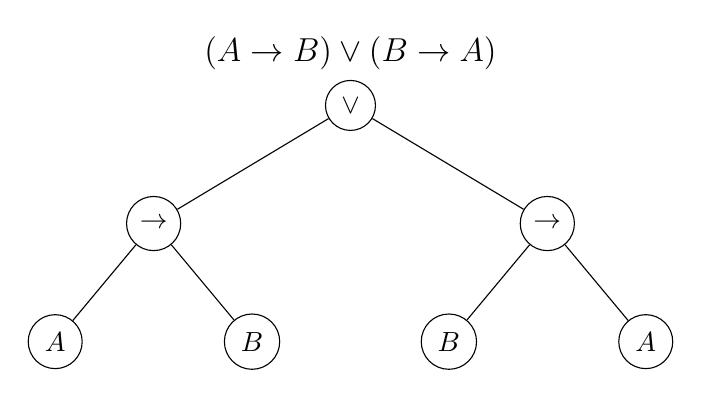
\begin{tikzpicture} [level/.style={sibling distance=50mm/#1}],
       \node [circle,draw] { $\lor$ }
         child { node [circle,draw] { $\to$ }
            child { node [circle,draw] { $A$ } }
            child { node [circle,draw] { $B$ } } }
         child { node [circle,draw] { $\to$ }
            child { node [circle,draw] { $B$ } } 
            child { node [circle,draw] { $A$ } } };
       \node[above,font=\large\bfseries] at (current bounding box.north) { $(A \to B) \lor (B \to A)$ };
    \end{tikzpicture}
    \end{figure}
\end{homeworkProblem}
\end{document}
